%FOR PDFLATEX USE ONLY
\documentclass[a4paper,12pt]{article}

\usepackage{amssymb,amsmath} %math symbols

\usepackage[margin=2cm]{geometry} %paper geometry

\usepackage[utf8]{inputenc} %allows unicode (including russian) source file
\usepackage[russian]{babel} %docment in russian-style
\usepackage[utf8]{inputenc}
%\usepackage[unicode]{hyperref} %links inside of the text
\usepackage[pdftex]{graphicx} %includegraphics pictures
\usepackage{cmlgc} %bold text

\usepackage{array} %arrays

%\usepackage{wrapfig}
%\usepackage{array}
%\usepackage{lipsum}
%\usepackage{esvect}
%\usepackage{hyperref}

\usepackage{subfig}
%\usepackage{calc}
%\usepackage{pgfplots,tikz,circuitikz}
%\usepackage{tkz-euclide}

\begin{document}

\begin{center}
  \LARGE{Работа 3.4.1}\\[0.2cm]
  \LARGE{диа- и парамагнетики}\\[0.2cm]
  \large{Малиновский Владимир}\\[0.2cm]
  \normalsize{\texttt{galqiwi@galqiwi.ru}}
\end{center}

\textbf{Цель работы:} измерение магнитной восприимчивости диа- и пара- магнитного образцов.\\
\textbf{В работе используются:} электромагнит, аналитические весы, милливеберметр, амперметр постоянного тока, реостаты и образцы.\\
\section*{Идея}

Если поместить стержень, состоящий из какого-то вещества в постоянное магнитное поле, на него начнет действовать сила:
$$F = \frac{\chi B^2 s}{2\mu_0},$$
где $F$ -- втягивающая сила, $s$ -- площадь сечения образца, $B$ -- напряженность магнитного поля, $\chi$ -- магнитная восприимчивость образца.

\begin{center}
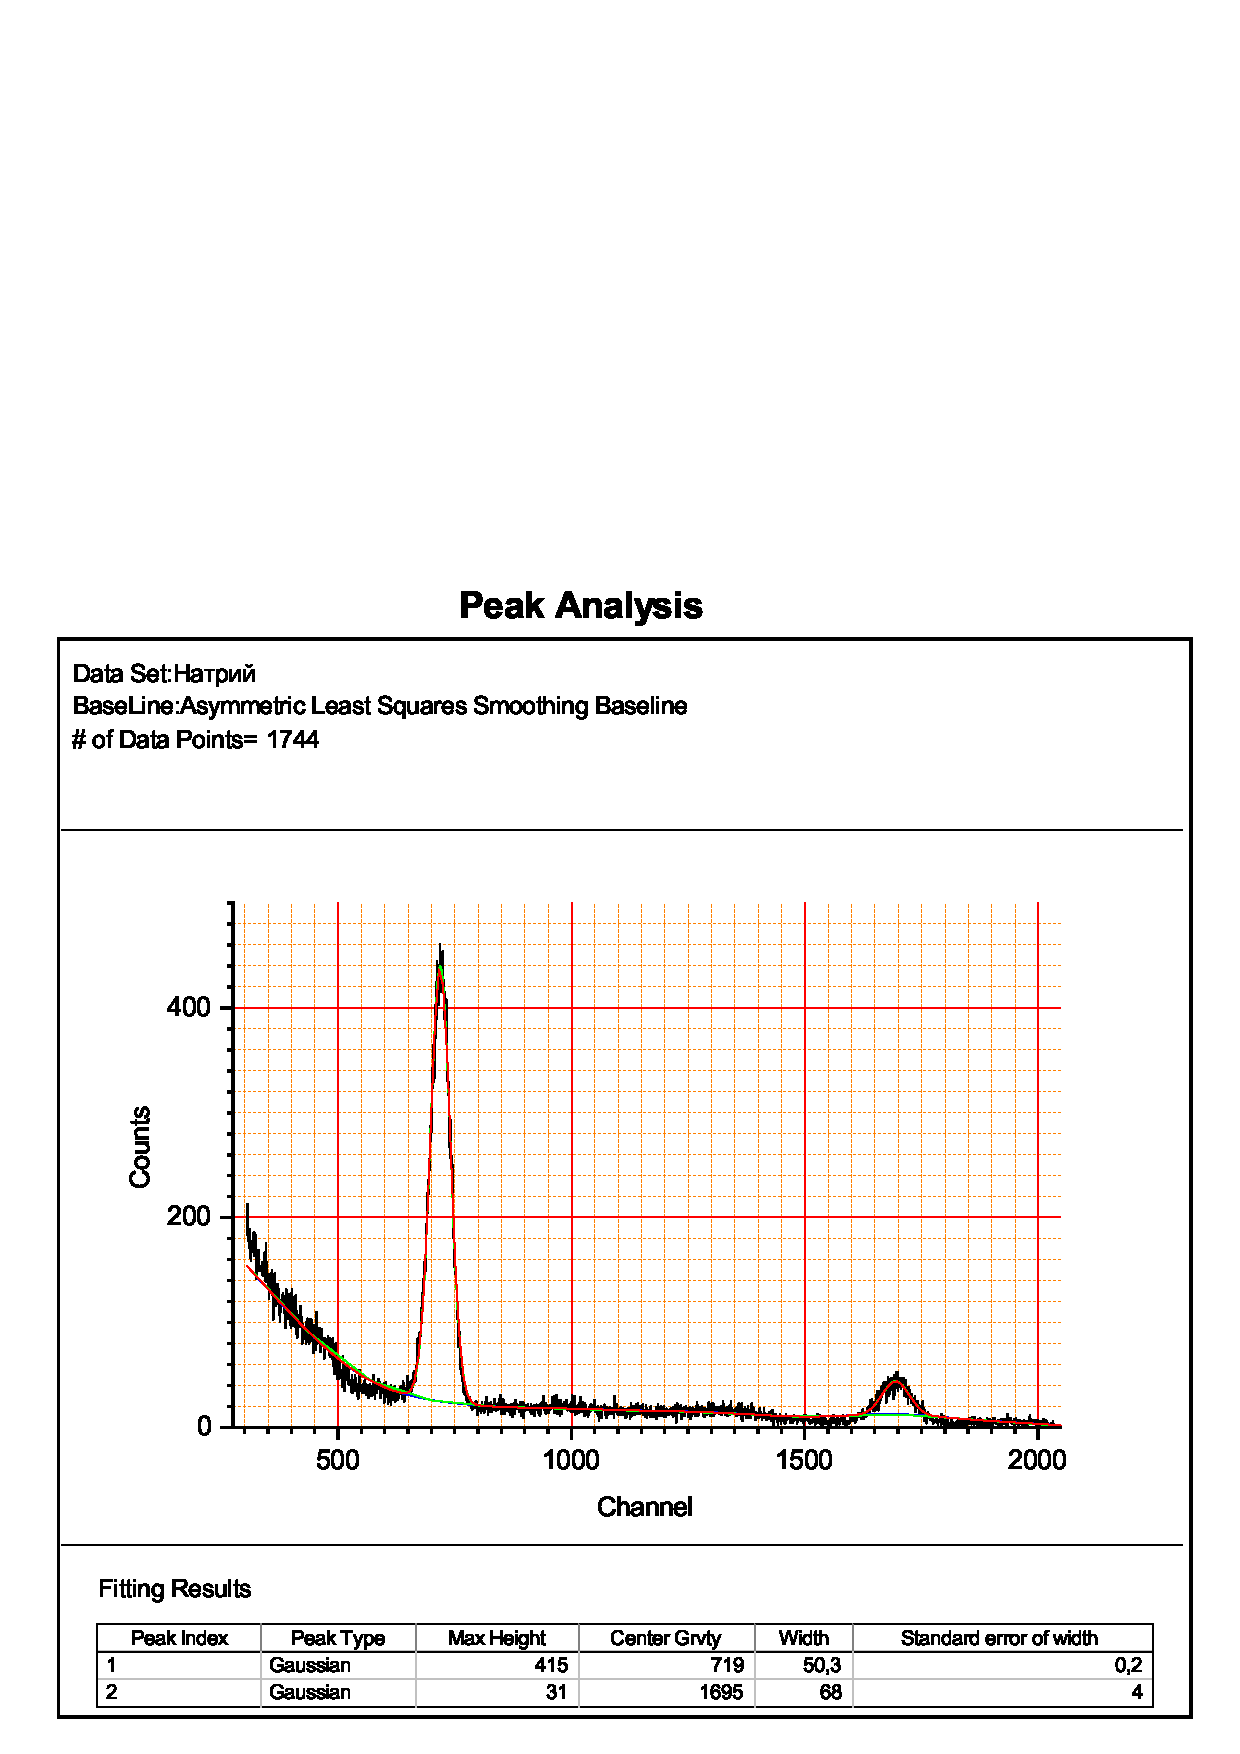
\includegraphics[width=0.40\textwidth]{1.png}
\end{center}

Если мы знаем $B$ и $F$, мы можем узнать $\chi$, что мы и сделаем.

\newpage
\section*{Методика и результаты}
Нумерация соответствует нумерации в лабнике.
\subsection*{1-2}
\begin{center}
\includegraphics[width=0.90\textwidth]{setup.png}
\end{center}
Проведем калибровку. Измерим зависимость магнитного потока $\Phi$, проходящего через милливеберметр с площадью $s_0 = 72\text{см}^2$ от тока, проходящего через электромагнит:
\begin{center}
\begin{tabular}{|c|c|c|}\hline
$I\text{, А}$&$F\text{, мВб}$&$B\text{, мТл}$\\\hline
$0.000$&$0.10$&$14$\\\hline
$0.170$&$1.50$&$208$\\\hline
$0.330$&$2.60$&$361$\\\hline
$0.500$&$3.90$&$542$\\\hline
$0.660$&$5.20$&$722$\\\hline
$0.830$&$6.30$&$875$\\\hline
$1.000$&$7.40$&$1028$\\\hline
$1.170$&$8.10$&$1125$\\\hline
\end{tabular}\\~\\
$\Delta I=0.005\,\text{А}, \Delta F=0.05\,\text{мВб}, \Delta B=7\,\text{мТл}$
\end{center}



\begin{center}
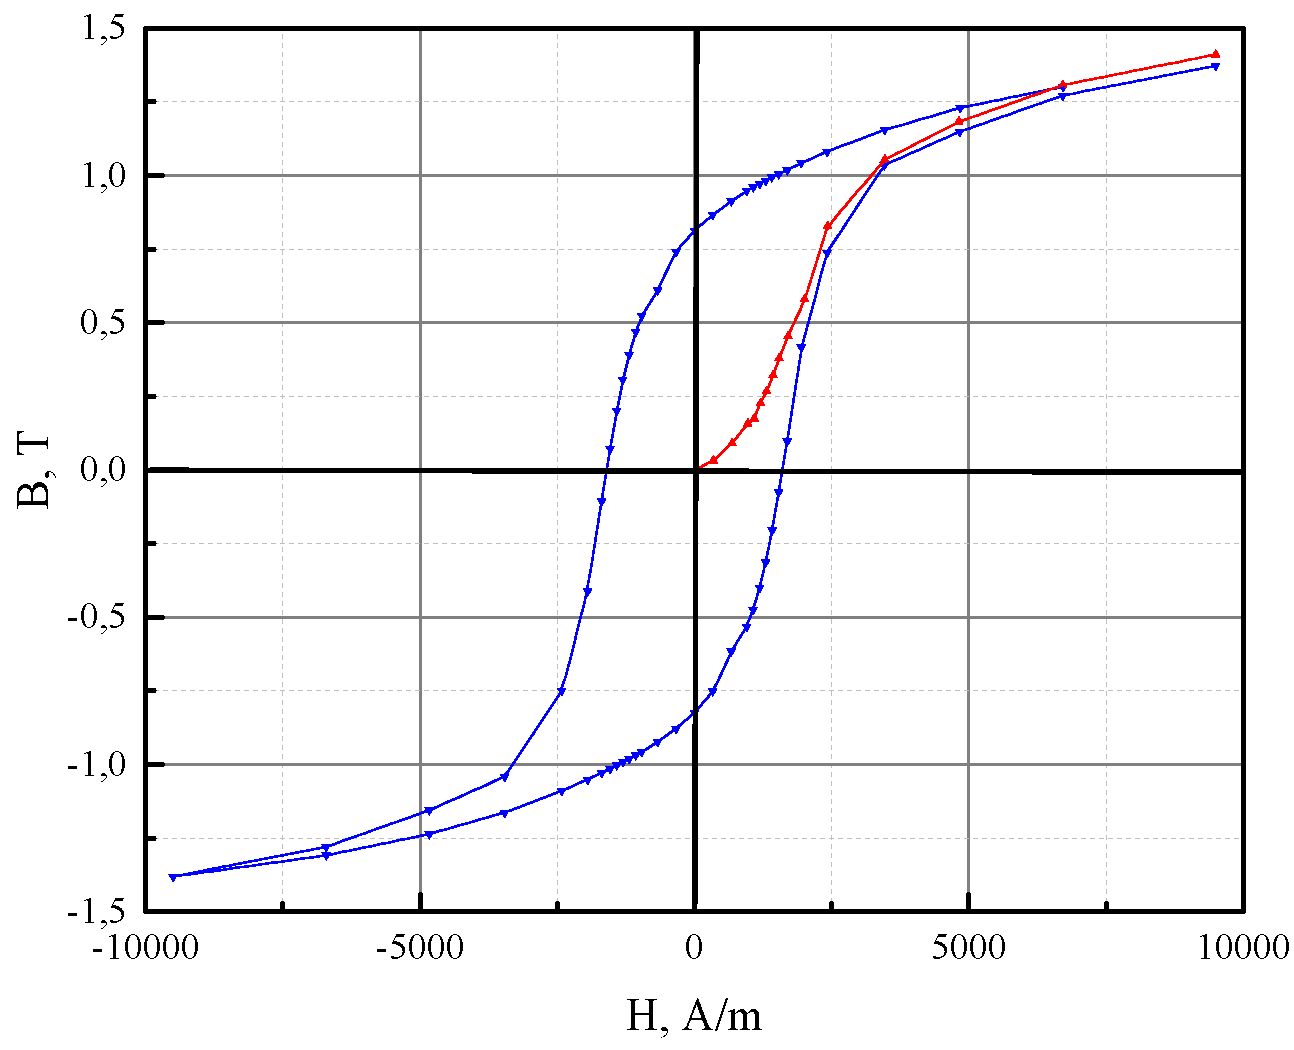
\includegraphics[width=0.90\textwidth]{plot.png}
\end{center}

Индукция поля $B$ находится как $\Phi/s_0$.\\
Как видно из графика, зависимость почти линейная. По МНК
$$B = K I,$$
где $K = (1.02\pm0.02)\,\frac{\text{Тл}}{\text{А}}$.
Но из-за того, что зависимость нелинейная, мы не можем просто использовать эту формулу. В дальнейшем я буду использовать значения тока, численно равные значениям тока, используемым при калибровке. Считая напряженность поля такой же, как при калибровке, ее погрешность будет
$$\sqrt{(\Delta B)^2 + (K \Delta{I})^2} = 0.009\,\text{Тл}.$$

\subsection*{3-5}
Для каждого образца я проарретировал весы и подвесил образец между магнитами. После этого я обнулил весы и подавал различные токи $I$ на электромагнит, выписывая показания весов, сначала увеличивая $I$, а потом уменьшая. Данные на странице 4.

\newpage
\subsection*{обработка-1-2}
Построим графики $\Delta m$ от $B^2$ и найдем $\chi$ из угла наклона.

\begin{center}
Алюминий\\~\\
\begin{tabular}{|c|c|c|c|c|c|}\hline
$I\text{, A}$&$B\text{, Тл}$&$B^2\text{, Тл}^2$&$\Delta B^2\text{, Тл}^2$&$m_{up}\text{, мг}$&$m_{down}\text{, мг}$\\\hline
$0.00$&$0.014$&$0.0002$&$0.0003$&$0.0$&$2.0$\\\hline
$0.17$&$0.208$&$0.043$&$0.004$&$3.0$&$3.0$\\\hline
$0.33$&$0.361$&$0.130$&$0.007$&$10.0$&$11.0$\\\hline
$0.50$&$0.542$&$0.29$&$0.01$&$19.0$&$20.0$\\\hline
$0.66$&$0.722$&$0.522$&$0.013$&$31.0$&$32.0$\\\hline
$0.83$&$0.875$&$0.766$&$0.016$&$45.0$&$47.0$\\\hline
$1.00$&$1.028$&$1.056$&$0.019$&$60.0$&$59.0$\\\hline
$1.17$&$1.125$&$1.27$&$0.02$&$71.0$&$71.0$\\\hline
\end{tabular}\\~\\
$\Delta I=0.01\,\text{A}, \Delta B=0.009\,\text{Тл}, \Delta m_{up}=0.5\,\text{мг}, \Delta m_{down}=0.5\,\text{мг}$
\end{center}

\begin{center}
Медь\\~\\
\begin{tabular}{|c|c|c|c|c|c|}\hline
$I\text{, A}$&$B\text{, Тл}$&$B^2\text{, Тл}^2$&$\Delta B^2\text{, Тл}^2$&$m_{up}\text{, мг}$&$m_{down}\text{, мг}$\\\hline
$0.00$&$0.014$&$0.0002$&$0.0003$&$1.0$&$0.0$\\\hline
$0.17$&$0.208$&$0.043$&$0.004$&$0.0$&$-3.0$\\\hline
$0.33$&$0.361$&$0.130$&$0.007$&$-3.0$&$-5.0$\\\hline
$0.50$&$0.542$&$0.29$&$0.01$&$-6.0$&$-9.0$\\\hline
$0.66$&$0.722$&$0.522$&$0.013$&$-11.0$&$-15.0$\\\hline
$0.83$&$0.875$&$0.766$&$0.016$&$-18.0$&$-21.0$\\\hline
$1.00$&$1.028$&$1.056$&$0.019$&$-26.0$&$-26.0$\\\hline
$1.17$&$1.125$&$1.27$&$0.02$&$-31.0$&$-32.0$\\\hline
\end{tabular}\\~\\
$\Delta I=0.01\,\text{A}, \Delta B=0.009\,\text{Тл}, \Delta m_{up}=0.5\,\text{мг}, \Delta m_{down}=0.5\,\text{мг}$
\end{center}

\begin{center}
Графит\\~\\
\begin{tabular}{|c|c|c|c|c|c|}\hline
$I\text{, A}$&$B\text{, Тл}$&$B^2\text{, Тл}^2$&$\Delta B^2\text{, Тл}^2$&$m_{up}\text{, мг}$&$m_{down}\text{, мг}$\\\hline
$0.00$&$0.014$&$0.0002$&$0.0003$&$0.0$&$-3.0$\\\hline
$0.17$&$0.208$&$0.043$&$0.004$&$38.0$&$31.0$\\\hline
$0.33$&$0.361$&$0.130$&$0.007$&$83.0$&$85.0$\\\hline
$0.50$&$0.542$&$0.29$&$0.01$&$136.0$&$140.0$\\\hline
$0.66$&$0.722$&$0.522$&$0.013$&$184.0$&$179.0$\\\hline
$0.83$&$0.875$&$0.766$&$0.016$&$229.0$&$226.0$\\\hline
$1.00$&$1.028$&$1.056$&$0.019$&$264.0$&$260.0$\\\hline
$1.17$&$1.125$&$1.27$&$0.02$&$288.0$&$283.0$\\\hline
\end{tabular}\\~\\
$\Delta I=0.01\,\text{A}, \Delta B=0.009\,\text{Тл}, \Delta m_{up}=0.5\,\text{мг}, \Delta m_{down}=0.5\,\text{мг}$
\end{center}
$\Delta B^2=2B\Delta B$

\newpage
Алюминий и Медь:
\begin{center}
\includegraphics[width=0.90\textwidth]{al-cu.png}
\end{center}

Из МНК:
$$m = K_1 B^2$$

$$K_{1al} = \frac{(57.3\pm0.8) + (57.7\pm1.3)}{2}\frac{\text{мг}}{\text{Тл}^2}=(57.5\pm1.6)\frac{\text{мг}}{\text{Тл}^2}$$

$$K_{1cu} = \frac{(-24.0\pm0.5) + (-25.9\pm0.7)}{2}\frac{\text{мг}}{\text{Тл}^2}=(-25.0\pm0.6)\frac{\text{мг}}{\text{Тл}^2}$$

$$\chi = \frac{2 \mu_0 K g} {s} = \frac{2 \mu_0 K g} {\pi d^2/4} ,$$
где $g$ -- ускорение свободного падения, $s$ -- площадь образца. $d_{al}=d_{cu}=d_{c}=1\,\text{см},$ где $d$ -- диаметр.

Из этого
$$\chi_{al} = (1.81\pm0.05)\,10^{-5}$$
$$\chi_{cu} = (-7.85\pm0.19)\,10^{-6}$$
При этом табличные значения:
$$\chi_{al} = (2.3)\,10^{-5}$$
$$\chi_{cu} = (-6.4\,\text{или}-9.2)\,10^{-6}$$

Мы правильно получили то, что медь диамагнетик, а алюминий парамагнетик. 

\newpage

Графит:
\begin{center}
\includegraphics[width=0.90\textwidth]{c.png}
\end{center}

Видно, что график $m$ от $B^2$ у графита нелинейный. Это значит, что в силе, прикладываемой к графиту максимальный вклад вносит не та сила, которую мы ожидали, и наша модель неприменима.

\section*{Вывод}
С помощью метода Гюи мы измерили магнитную восприимчивость меди и алюминия и поняли, что медь диамагнетик, а алюминий парамагнетик. Магнитная восприимчивость аллюминия отличается не больше, чем на $22\%$ от табличной, а восприимчивость меди лежит между двумя табличными значениями из различных источников. Промерить магнитную восприимчивость графита этим методом не вышло, поскольку в реальной установке возникают неизвестные пока мне эффекты, которые мы не учитываем в модели.
\end{document}


125





\lipsum[1-4]
\begin{wrapfigure}{R}{5cm}
\centering
\includegraphics[width=0.20\textwidth]{rd.png}
\caption{1}
\end{wrapfigure}
\lipsum[1-6]


\begin{figure}[h]
\begin{center}$
\begin{array}{cccc}
\includegraphics[width=0.20\textwidth]{rd.png}&
\includegraphics[width=0.20\textwidth]{rd.png}&
\includegraphics[width=0.20\textwidth]{rd.png}&
\includegraphics[width=0.20\textwidth]{rd.png}\\
(1) & (2) & (3) & (4)
\end{array}$
\end{center}
\end{figure}
